\documentclass[tikz,border=0pt]{standalone}
\pdfminorversion=7
\usepackage[T1]{fontenc}
\usepackage{lmodern,amsmath,amssymb,graphicx}
\usepackage{pgfplots}
\usetikzlibrary{arrows.meta,calc,positioning,patterns,decorations.pathreplacing}
\pgfplotsset{compat=1.18}
\definecolor{family}{RGB}{0,140,18}
\definecolor{familypale}{RGB}{225,255,226}
\definecolor{frozen}{RGB}{49,57,208}
\definecolor{frozenpale}{RGB}{234,235,255}
\definecolor{adapter}{RGB}{219,102,0}
\definecolor{adapterpale}{RGB}{255,196,135}
\definecolor{outputcol}{RGB}{120,38,130}
\definecolor{ink}{RGB}{33,33,33}
\definecolor{muted}{RGB}{105,105,105}
\tikzset{
 figure/.style={x=1pt,y=1pt,line cap=round,line join=round,text=ink,
   >={Stealth[length=7pt,width=6pt]},font=\fontsize{20}{24}\selectfont},
 title/.style={font=\fontsize{29}{33}\selectfont},
 heading/.style={font=\fontsize{22}{26}\selectfont},
 labeltext/.style={font=\fontsize{18}{22}\selectfont,align=center},
 smalllabel/.style={font=\fontsize{15}{19}\selectfont,align=center},
 equation/.style={font=\fontsize{24}{29}\selectfont,align=center},
 flow/.style={->,line width=1.3pt},
 fineflow/.style={->,line width=.8pt},
 target/.style={circle,fill=family,draw=white,line width=1.2pt,inner sep=0pt,minimum size=12pt},
 candidate/.style={circle,fill=white,draw=muted,line width=1.3pt,inner sep=0pt,minimum size=10pt},
 neuron/.style={circle,draw=frozen,fill=frozen!18,minimum size=13pt,inner sep=0pt,line width=.8pt}
}
\DeclareMathOperator{\rank}{rank}
\DeclareMathOperator{\row}{row}
\DeclareMathOperator{\col}{col}
\newcommand{\R}{\mathbb R}
\graphicspath{{assets/}}
\newcommand{\canvas}[1]{\path[use as bounding box] (0,0) rectangle (960,600);
  \node[title,anchor=west] at (36,557) {#1};}
\newcommand{\glyphgrid}[2]{
 \begin{scope}[shift={(#1,#2)}]
  \fill[white] (0,0) rectangle (136,136);
  \foreach \x/\y/\c in {1/1/80,2/2/80,2/3/45,3/4/45,3/5/45,4/5/100,4/6/45,5/6/45,5/4/45,5/2/100,6/1/80}{
    \fill[frozen!\c] (\x*17,\y*17) rectangle ++(17,17);
  }
  \draw[step=17pt,black!30,line width=.35pt] (0,0) grid (136,136);
  \draw[black!45,line width=.6pt] (0,0) rectangle (136,136);
 \end{scope}}

\begin{document}
\begin{tikzpicture}[figure]
\canvas{MNIST and the image family}
\node[smalllabel,text=muted,anchor=east] at (922,557) {Replay diagnostic};
\node[labeltext,text=muted] at (480,514) {Original / reconstruction};
\node[heading,anchor=west] at (49,468) {Public PCA};
\node[inner sep=0pt] at (480,410) {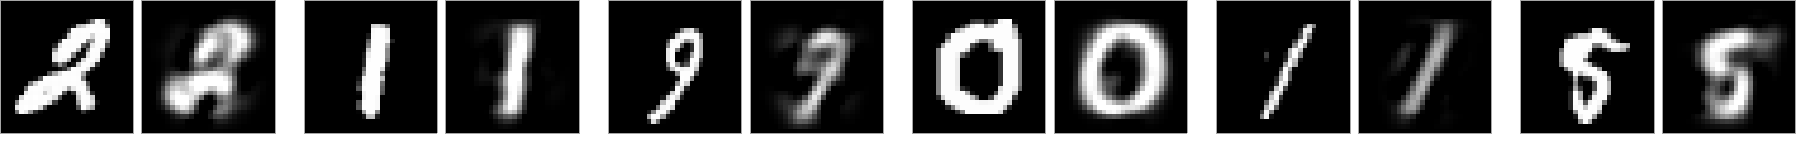
\includegraphics[width=866pt]{mnist_gt_2.pdf}};
\node[heading,anchor=west] at (49,327) {Warped family};
\node[inner sep=0pt] at (480,269) {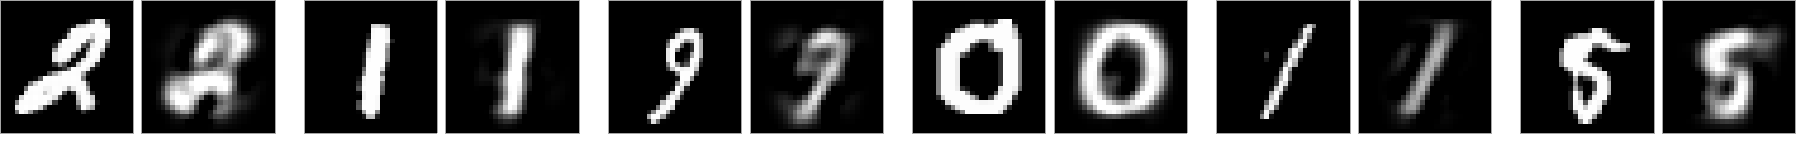
\includegraphics[width=866pt]{mnist_gt_3.pdf}};
\node[heading,anchor=west] at (49,186) {Private-built reference};
\node[inner sep=0pt] at (480,128) {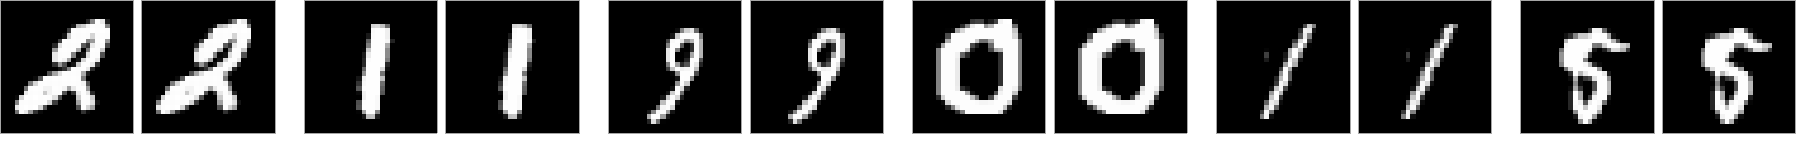
\includegraphics[width=866pt]{mnist_gt_4.pdf}};
\node[smalllabel,text=muted] at (480,35) {Separate represented targets};
\end{tikzpicture}
\end{document}
